\documentclass{article}
\usepackage[utf8]{inputenc}
\usepackage[a1paper,landscape,margin=2cm]{geometry}
\usepackage{graphicx}
\usepackage{xcolor}
\usepackage{tikz}
\usepackage{array}
\usepackage{colortbl}

\definecolor{bluebg}{HTML}{90CAF9}
\definecolor{bluetext}{HTML}{0D47A1}
\definecolor{orangebg}{HTML}{FFCC80}
\definecolor{orangetext}{HTML}{E65100}
\definecolor{greenbg}{HTML}{A5D6A7}
\definecolor{greentext}{HTML}{1B5E20}
\definecolor{redbg}{HTML}{EF9A9A}
\definecolor{redtext}{HTML}{B71C1C}
\definecolor{purplebg}{HTML}{CE93D8}
\definecolor{purpletext}{HTML}{4A148C}
\definecolor{yellowbg}{HTML}{FFF59D}
\definecolor{yellowtext}{HTML}{F57F17}
\definecolor{tealbg}{HTML}{80CBC4}
\definecolor{tealtext}{HTML}{004D40}
\definecolor{pinkbg}{HTML}{F48FB1}
\definecolor{pinktext}{HTML}{880E4F}
\definecolor{graybg}{HTML}{BDBDBD}

\begin{document}
\pagestyle{empty}

\begin{center}
{\fontsize{56}{66}\selectfont\bfseries\color{bluetext} TASI Intraday Trading System}\\[0.5cm]
{\fontsize{32}{38}\selectfont Horizontal Timeline Process Map --- Version 4.0}\\[0.2cm]
{\fontsize{24}{28}\selectfont May 21, 2026 --- Saudi Exchange (Tadawul)}\\[1.5cm]
\end{center}

% Main horizontal timeline
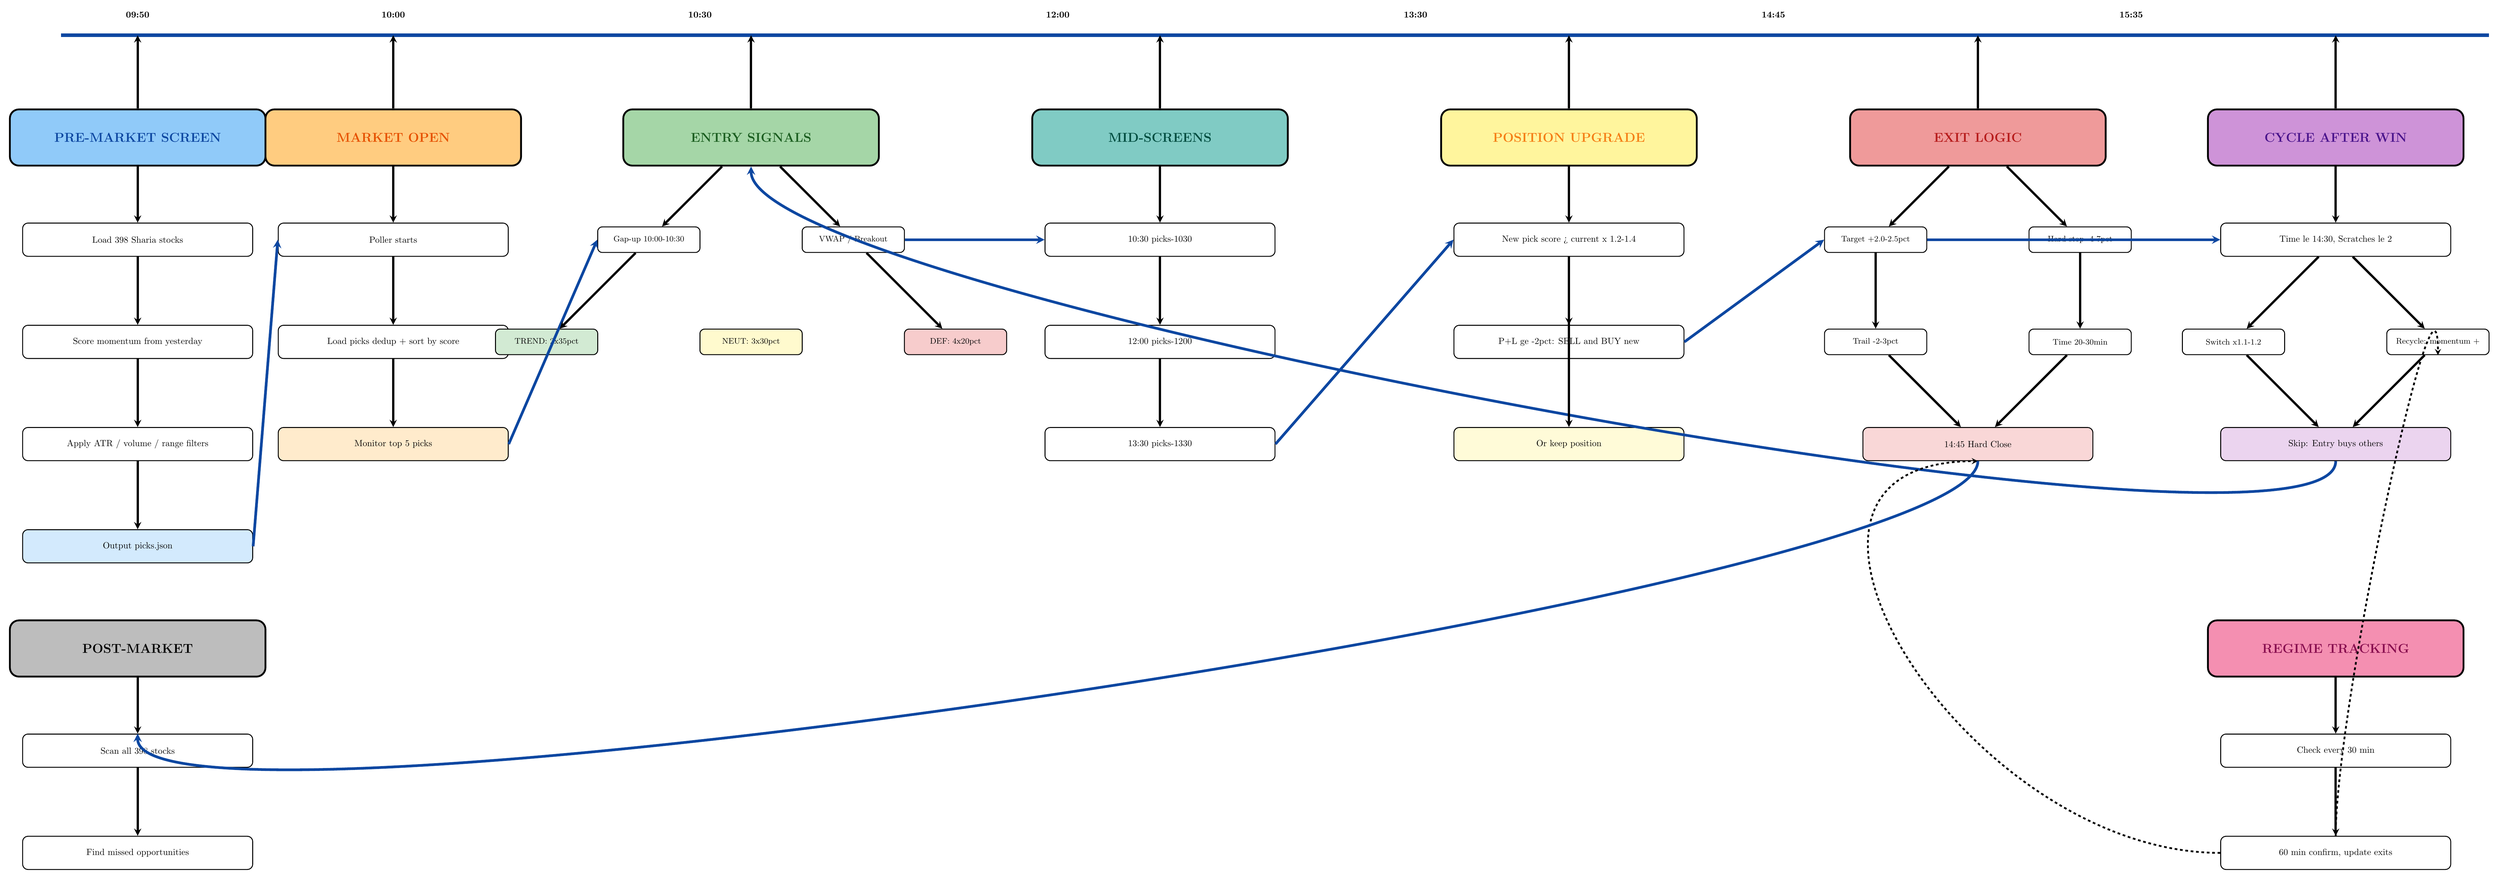
\begin{tikzpicture}[
    timeline/.style={draw, line width=4pt, color=bluetext},
    stagebox/.style={draw, line width=2pt, rounded corners=10pt, minimum width=10cm, minimum height=2.2cm, align=center, font=\Large\bfseries},
    detailbox/.style={draw, line width=1pt, rounded corners=6pt, minimum width=9cm, minimum height=1.3cm, align=center, font=\normalsize},
    subbox/.style={draw, line width=1pt, rounded corners=5pt, minimum width=4cm, minimum height=1cm, align=center, font=\small},
    arrow/.style={->, >=stealth, line width=2.5pt},
    dasharrow/.style={->, >=stealth, line width=2pt, dashed},
    timearrow/.style={->, >=stealth, line width=3pt, color=bluetext}
]

% =============================================
% MAIN TIMELINE (horizontal across top)
% =============================================
\draw[timeline] (-15, 10) -- (80, 10);

% Time markers
\foreach \x/\time in {-12/09:50, -2/10:00, 10/10:30, 24/12:00, 38/13:30, 52/14:45, 66/15:35}
    \node[font=\bfseries] at (\x, 10.8) {\time};

% =============================================
% STAGE 1: PRE-MARKET (leftmost)
% =============================================
\node[stagebox, fill=bluebg, text=bluetext] (pm) at (-12, 6) {PRE-MARKET SCREEN};
\node[detailbox, fill=white] (pm1) at (-12, 2) {Load 398 Sharia stocks};
\node[detailbox, fill=white] (pm2) at (-12, -2) {Score momentum from yesterday};
\node[detailbox, fill=white] (pm3) at (-12, -6) {Apply ATR / volume / range filters};
\node[detailbox, fill=bluebg!40] (pm4) at (-12, -10) {Output picks.json};

% Vertical connector to timeline
\draw[arrow] (pm) -- (-12, 10);

% =============================================
% STAGE 2: MARKET OPEN
% =============================================
\node[stagebox, fill=orangebg, text=orangetext] (mo) at (-2, 6) {MARKET OPEN};
\node[detailbox, fill=white] (mo1) at (-2, 2) {Poller starts};
\node[detailbox, fill=white] (mo2) at (-2, -2) {Load picks dedup + sort by score};
\node[detailbox, fill=orangebg!40] (mo3) at (-2, -6) {Monitor top 5 picks};

\draw[arrow] (mo) -- (-2, 10);

% =============================================
% STAGE 3: ENTRY (center)
% =============================================
\node[stagebox, fill=greenbg, text=greentext] (en) at (12, 6) {ENTRY SIGNALS};
\node[subbox, fill=white] (en1) at (8, 2) {Gap-up 10:00-10:30};
\node[subbox, fill=white] (en2) at (16, 2) {VWAP / Breakout};

% Regime sizing
\node[subbox, fill=greenbg!50] (rs1) at (4, -2) {TREND: 2x35pct};
\node[subbox, fill=yellowbg!50] (rs2) at (12, -2) {NEUT: 3x30pct};
\node[subbox, fill=redbg!50] (rs3) at (20, -2) {DEF: 4x20pct};

\draw[arrow] (en) -- (12, 10);

% =============================================
% STAGE 4: MID-SCREENS
% =============================================
\node[stagebox, fill=tealbg, text=tealtext] (ms) at (28, 6) {MID-SCREENS};
\node[detailbox, fill=white] (ms1) at (28, 2) {10:30 picks-1030};
\node[detailbox, fill=white] (ms2) at (28, -2) {12:00 picks-1200};
\node[detailbox, fill=white] (ms3) at (28, -6) {13:30 picks-1330};

\draw[arrow] (ms) -- (28, 10);

% =============================================
% STAGE 5: POSITION UPGRADE (below mid-screens)
% =============================================
\node[stagebox, fill=yellowbg, text=yellowtext] (pu) at (44, 6) {POSITION UPGRADE};
\node[detailbox, fill=white] (pu1) at (44, 2) {New pick score > current x 1.2-1.4};
\node[detailbox, fill=white] (pu2) at (44, -2) {P+L ge -2pct: SELL and BUY new};
\node[detailbox, fill=yellowbg!40] (pu3) at (44, -6) {Or keep position};

\draw[arrow] (pu) -- (44, 10);

% =============================================
% STAGE 6: EXIT (far right top)
% =============================================
\node[stagebox, fill=redbg, text=redtext] (ex) at (60, 6) {EXIT LOGIC};
\node[subbox, fill=white] (ex1) at (56, 2) {Target +2.0-2.5pct};
\node[subbox, fill=white] (ex2) at (64, 2) {Hard stop -4-7pct};
\node[subbox, fill=white] (ex3) at (56, -2) {Trail -2-3pct};
\node[subbox, fill=white] (ex4) at (64, -2) {Time 20-30min};
\node[detailbox, fill=redbg!40] (ex5) at (60, -6) {14:45 Hard Close};

\draw[arrow] (ex) -- (60, 10);

% =============================================
% STAGE 7: CYCLE (far right)
% =============================================
\node[stagebox, fill=purplebg, text=purpletext] (cy) at (74, 6) {CYCLE AFTER WIN};
\node[detailbox, fill=white] (cy1) at (74, 2) {Time le 14:30, Scratches le 2};
\node[subbox, fill=white] (cy2) at (70, -2) {Switch x1.1-1.2};
\node[subbox, fill=white] (cy3) at (78, -2) {Recycle: momentum +};
\node[detailbox, fill=purplebg!40] (cy4) at (74, -6) {Skip: Entry buys others};

\draw[arrow] (cy) -- (74, 10);

% =============================================
% STAGE 8: REGIME TRACKING (bottom right)
% =============================================
\node[stagebox, fill=pinkbg, text=pinktext] (rg) at (74, -14) {REGIME TRACKING};
\node[detailbox, fill=white] (rg1) at (74, -18) {Check every 30 min};
\node[detailbox, fill=white] (rg2) at (74, -22) {60 min confirm, update exits};

% =============================================
% STAGE 9: POST-MARKET (bottom left)
% =============================================
\node[stagebox, fill=graybg, text=black] (po) at (-12, -14) {POST-MARKET};
\node[detailbox, fill=white] (po1) at (-12, -18) {Scan all 398 stocks};
\node[detailbox, fill=white] (po2) at (-12, -22) {Find missed opportunities};

% =============================================
% FLOW ARROWS (horizontal, no overlaps)
% =============================================

% Pre-market to market open
\draw[timearrow] (pm4.east) -- (mo1.west);

% Market open to entry
\draw[timearrow] (mo3.east) -- (en1.west);

% Entry to mid-screens
\draw[timearrow] (en2.east) -- (ms1.west);

% Mid-screens to position upgrade
\draw[timearrow] (ms3.east) -- (pu1.west);

% Position upgrade to exit
\draw[timearrow] (pu2.east) -- (ex1.west);

% Exit target to cycle
\draw[timearrow] (ex1.east) -- (cy1.west);

% Cycle back to entry (curved under)
\draw[timearrow] (cy4.south) .. controls +(0,-5) and +(0,-5) .. (en.south);

% Regime influence (dashed, from bottom)
\draw[dasharrow] (rg2.west) .. controls +(-10,0) and +(-10,0) .. (ex5.south);
\draw[dasharrow] (rg2.north) .. controls +(0,5) and +(0,5) .. (cy3.south);

% Hard close to post-market (curved under)
\draw[timearrow] (ex5.south) .. controls +(0,-5) and +(0,-5) .. (po1.north);

% =============================================
% INTERNAL VERTICAL FLOWS
% =============================================
\draw[arrow] (pm) -- (pm1);
\draw[arrow] (pm1) -- (pm2);
\draw[arrow] (pm2) -- (pm3);
\draw[arrow] (pm3) -- (pm4);

\draw[arrow] (mo) -- (mo1);
\draw[arrow] (mo1) -- (mo2);
\draw[arrow] (mo2) -- (mo3);

\draw[arrow] (en) -- (en1);
\draw[arrow] (en) -- (en2);
\draw[arrow] (en1) -- (rs1);
\draw[arrow] (en2) -- (rs3);

\draw[arrow] (ms) -- (ms1);
\draw[arrow] (ms1) -- (ms2);
\draw[arrow] (ms2) -- (ms3);

\draw[arrow] (pu) -- (pu1);
\draw[arrow] (pu1) -- (pu2);
\draw[arrow] (pu1) -- (pu3);

\draw[arrow] (ex) -- (ex1);
\draw[arrow] (ex) -- (ex2);
\draw[arrow] (ex1) -- (ex3);
\draw[arrow] (ex2) -- (ex4);
\draw[arrow] (ex3) -- (ex5);
\draw[arrow] (ex4) -- (ex5);

\draw[arrow] (cy) -- (cy1);
\draw[arrow] (cy1) -- (cy2);
\draw[arrow] (cy1) -- (cy3);
\draw[arrow] (cy2) -- (cy4);
\draw[arrow] (cy3) -- (cy4);

\draw[arrow] (rg) -- (rg1);
\draw[arrow] (rg1) -- (rg2);

\draw[arrow] (po) -- (po1);
\draw[arrow] (po1) -- (po2);

\end{tikzpicture}

\vspace{2cm}

\begin{center}
{\fontsize{28}{34}\selectfont\bfseries Color Legend}\\[0.8cm]
\begin{tabular}{|c|c|c|c|c|c|c|c|c|}
\hline
\cellcolor{bluebg}\textbf{\color{bluetext}Pre-Market} & 
\cellcolor{orangebg}\textbf{\color{orangetext}Market} & 
\cellcolor{greenbg}\textbf{\color{greentext}Entry} & 
\cellcolor{tealbg}\textbf{\color{tealtext}Mid-Screen} & 
\cellcolor{yellowbg}\textbf{\color{yellowtext}Upgrade} & 
\cellcolor{redbg}\textbf{\color{redtext}Exit} & 
\cellcolor{purplebg}\textbf{\color{purpletext}Cycle} & 
\cellcolor{pinkbg}\textbf{\color{pinktext}Regime} & 
\cellcolor{graybg}\textbf{Post} \\
\hline
09:50 & 10:00 & 10:00-10:30 & 10:30/12/13:30 & 10:30/12/13:30 & All day & After win & Every 30min & 15:35 \\
\hline
\end{tabular}
\end{center}

\end{document}
